\documentclass[12pt,a4paper,oneside]{report}

% ---------------------------------------------------------------------------
% FONTS -- Times New Roman substitute (TeX Gyre Termes) + Courier substitute
% ---------------------------------------------------------------------------
% \usepackage{fontspec}
% \setmainfont{TeX Gyre Termes}
% \setmonofont{TeX Gyre Cursor}[Scale=0.92]
\usepackage{mathptmx}
\usepackage{courier}
\usepackage[T1]{fontenc}

% ---------------------------------------------------------------------------
% PAGE GEOMETRY -- A4, 1in margins, 1.5in binding edge
% ---------------------------------------------------------------------------
\usepackage[a4paper,left=1.5in,right=1in,top=1in,bottom=1in,headheight=15pt]{geometry}

% ---------------------------------------------------------------------------
% SPACING, JUSTIFICATION
% ---------------------------------------------------------------------------
\usepackage{setspace}
\onehalfspacing
\usepackage{ragged2e}
\usepackage{microtype}
\tolerance=1200
\emergencystretch=2.5em
\hbadness=3000
\hfuzz=2pt

% ---------------------------------------------------------------------------
% HEADERS / FOOTERS / PAGE NUMBERS
% ---------------------------------------------------------------------------
\usepackage{fancyhdr}
\pagestyle{fancy}
\fancyhf{}
\renewcommand{\headrulewidth}{0.4pt}
\fancyhead[L]{\nouppercase{\leftmark}}
\fancyhead[R]{\thepage}
\fancypagestyle{plain}{%
  \fancyhf{}
  \fancyhead[L]{\nouppercase{\leftmark}}
  \fancyhead[R]{\thepage}
  \renewcommand{\headrulewidth}{0.4pt}
}

% ---------------------------------------------------------------------------
% CHAPTER / SECTION HEADING STYLE (decimal numbering is report-class default)
% ---------------------------------------------------------------------------
\usepackage{titlesec}
\titleformat{\chapter}[display]
  {\normalfont\bfseries}{\Large CHAPTER \thechapter}{6pt}{\Huge}
\titlespacing*{\chapter}{0pt}{0pt}{28pt}
\titleformat{\section}{\normalfont\Large\bfseries}{\thesection}{10pt}{}
\titleformat{\subsection}{\normalfont\large\bfseries\itshape}{\thesubsection}{8pt}{}

% ---------------------------------------------------------------------------
% FIGURES / TABLES -- numbered within chapter, captions
% ---------------------------------------------------------------------------
\usepackage{graphicx}
\usepackage[labelfont=bf,font=small,margin=0.6cm]{caption}
\counterwithin{figure}{chapter}
\counterwithin{table}{chapter}
\usepackage{booktabs}
\usepackage{longtable}
\usepackage{array}
\usepackage{tabularx}
\newcolumntype{Y}{>{\raggedright\arraybackslash}X}

% ---------------------------------------------------------------------------
% CODE LISTINGS
% ---------------------------------------------------------------------------
\usepackage{listings}
\usepackage{xcolor}
\definecolor{codebg}{RGB}{243,243,243}
\definecolor{codecomment}{RGB}{90,90,90}
\definecolor{codestring}{RGB}{110,50,40}
\definecolor{coderule}{RGB}{60,80,100}

\lstdefinestyle{cstyle}{
  language=C,
  backgroundcolor=\color{codebg},
  basicstyle=\ttfamily\small,
  keywordstyle=\bfseries,
  commentstyle=\itshape\color{codecomment},
  stringstyle=\color{codestring},
  numbers=left,
  numberstyle=\tiny\color{codecomment},
  numbersep=8pt,
  frame=single,
  rulecolor=\color{coderule},
  framerule=0.4pt,
  breaklines=true,
  breakatwhitespace=false,
  showstringspaces=false,
  tabsize=2,
  columns=flexible,
  xleftmargin=1em,
  xrightmargin=0.3em,
  aboveskip=8pt,
  belowskip=8pt,
}

\lstdefinestyle{plainstyle}{
  backgroundcolor=\color{codebg},
  basicstyle=\ttfamily\small,
  numbers=left,
  numberstyle=\tiny\color{codecomment},
  numbersep=8pt,
  frame=single,
  rulecolor=\color{coderule},
  framerule=0.4pt,
  breaklines=true,
  breakatwhitespace=false,
  showstringspaces=false,
  tabsize=2,
  columns=flexible,
  xleftmargin=1em,
  xrightmargin=0.3em,
  aboveskip=8pt,
  belowskip=8pt,
}

\lstdefinestyle{mdstyle}{
  backgroundcolor=\color{codebg},
  basicstyle=\ttfamily\footnotesize,
  frame=single,
  rulecolor=\color{coderule},
  framerule=0.4pt,
  breaklines=true,
  breakatwhitespace=true,
  showstringspaces=false,
  columns=flexible,
  xleftmargin=1em,
  xrightmargin=0.3em,
  aboveskip=8pt,
  belowskip=8pt,
}

% ---------------------------------------------------------------------------
% LISTS
% ---------------------------------------------------------------------------
\usepackage{enumitem}
\setlist{topsep=4pt,itemsep=2pt,parsep=2pt}

% ---------------------------------------------------------------------------
% MISC
% ---------------------------------------------------------------------------
\usepackage{amsmath}
\usepackage{amssymb}
\usepackage{textcomp}
\usepackage[most]{tcolorbox}
\newtcolorbox{takeaway}{colback=gray!8,colframe=gray!50!black,boxrule=0.5pt,arc=1pt,left=6pt,right=6pt,top=4pt,bottom=4pt}

% ---------------------------------------------------------------------------
% HYPERLINKS (load near end of preamble)
% ---------------------------------------------------------------------------
\usepackage[hidelinks,pdfusetitle]{hyperref}
\hypersetup{
  colorlinks=false,
  pdfauthor={Author},
  pdfsubject={M.Tech Thesis},
  pdfkeywords={Embedded Systems, ARM Cortex-M7, STM32H7, Renode, RTOS, DMA, MAVLink, MPU}
}
\usepackage[nameinlink,capitalise]{cleveref}

% ---------------------------------------------------------------------------
% FRONT-MATTER TOC ENTRY HELPER (unnumbered chapters that still appear in ToC)
% ---------------------------------------------------------------------------
\newcommand{\frontchapter}[1]{%
  \chapter*{#1}
  \addcontentsline{toc}{chapter}{#1}
  \markboth{#1}{#1}
}

\begin{document}

% =============================================================================
% FRONT MATTER
% =============================================================================
\pagenumbering{roman}

\begin{titlepage}
\centering
\thispagestyle{empty}

\vspace*{0.5cm}
{\large\bfseries DETERMINISTIC RADAR-INERTIAL GEOREFERENCING COPROCESSOR\par}
\vspace{0.15cm}
{\large\bfseries ON STM32H7 (ARM CORTEX-M7):\par}
\vspace{0.15cm}
{\normalsize BARE-METAL FIRMWARE DESIGN AND RENODE HARDWARE-IN-THE-LOOP VERIFICATION\par}

\vspace{2.2cm}
{\normalsize A thesis submitted in partial fulfilment of the requirements for the degree of\par}
\vspace{0.3cm}
{\large\bfseries MASTER OF TECHNOLOGY IN EMBEDDED SYSTEMS\par}

\vspace{1.6cm}
{\normalsize by\par}
\vspace{0.25cm}
{\large\bfseries [AUTHOR FULL NAME]\par}
\vspace{0.15cm}
{\normalsize [ROLL / REGISTRATION NUMBER]\par}

\vspace{1.6cm}
{\normalsize Supervisor\par}
\vspace{0.2cm}
{\large\bfseries [SUPERVISOR FULL NAME, DESIGNATION]\par}

\vfill
{\normalsize [MONTH, YEAR OF SUBMISSION]\par}
\vspace{0.3cm}

\end{titlepage}
\frontchapter{Certificate}

This is to certify that the thesis entitled \textbf{``Bridging the Simulator--Silicon Gap: Progressive Design and Renode-Verified Hardening of a Fault-Resilient Telemetry Firmware Stack on the STM32H7 (Arm Cortex-M7)''}, submitted by \textbf{[AUTHOR FULL NAME]} (Registration No. \textbf{[ROLL / REGISTRATION NUMBER]}) in partial fulfilment of the requirements for the award of the degree of \textbf{[DEGREE NAME]} of \textbf{[UNIVERSITY / INSTITUTION NAME]}, is a bona fide record of the work carried out by the candidate under my supervision. The matter embodied in this thesis has not been submitted, in part or in full, to any other university or institute for the award of any other degree or diploma.

\vspace{2.2cm}
\noindent
\begin{minipage}[t]{0.45\textwidth}
[Place] \\{}
[Date]
\end{minipage}%
\begin{minipage}[t]{0.45\textwidth}
\raggedleft
\rule{6cm}{0.4pt}\\
\textbf{[SUPERVISOR FULL NAME]} \\{}
[Supervisor Designation] \\{}
[Department, Institution]
\end{minipage}

\frontchapter{Declaration}

I declare that this thesis titled \textbf{``Bridging the Simulator--Silicon Gap: Progressive Design and Renode-Verified Hardening of a Fault-Resilient Telemetry Firmware Stack on the STM32H7 (Arm Cortex-M7)''} and the work presented in it are my own. I confirm that:

\begin{itemize}
\item This work was done wholly during candidature for a research degree at \textbf{[UNIVERSITY / INSTITUTION NAME]}.
\item Where I have consulted the published work of others, this is always clearly attributed.
\item Where I have quoted from the work of others, the source is always given. With the exception of such quotations, this thesis is entirely my own work.
\item I have acknowledged all main sources of help.
\item All firmware, simulation scripts, and engineering logs described in Chapters 3--5 and reproduced in Appendices A--E were authored and verified by me on the stated toolchain (\texttt{arm-none-eabi-gcc}) and verification platform (Renode), with the single physical-hardware confirmation explicitly identified as such in Section 5.2.
\end{itemize}

\vspace{2.0cm}
\noindent
\begin{minipage}[t]{0.45\textwidth}
[Place] \\{}
[Date]
\end{minipage}%
\begin{minipage}[t]{0.45\textwidth}
\raggedleft
\rule{6cm}{0.4pt}\\
\textbf{[AUTHOR FULL NAME]} \\{}
[Roll / Registration Number]
\end{minipage}

\frontchapter{Acknowledgement}

I would like to express my sincere gratitude to my supervisor, \textbf{[SUPERVISOR FULL NAME]}, for the guidance, patience, and technical scrutiny extended throughout this project, and in particular for pressing me to distinguish, at every stage, between what the simulator had actually shown me and what I merely believed to be true of the hardware. I am grateful to the faculty and staff of \textbf{[DEPARTMENT NAME]}, \textbf{[UNIVERSITY / INSTITUTION NAME]}, for the laboratory access and physical STM32H753 hardware that made the Chapter 4 CRC-endianness confirmation possible. I would also like to thank the open-source communities behind Renode, the GNU Arm Embedded Toolchain, and the broader Cortex-M developer ecosystem, whose documentation and tooling this project depends on directly. Finally, I thank my family and friends for their patience and support during the long evenings this project's debugging sessions occasionally demanded.

\vspace{1.2cm}
\begin{flushright}
\textbf{[AUTHOR FULL NAME]}
\end{flushright}

\frontchapter{Abstract}

Drone-based radar search-and-rescue requires real-time spatial georeferencing: translating local radar detections into global GPS coordinates by fusing the drone's inertial state with radar range-Doppler measurements. This thesis presents the design and verification of a deterministic radar-inertial georeferencing coprocessor on the STM32H753 (Arm Cortex-M7), built entirely at the bare-metal register level and verified using Antmicro's open-source Renode functional simulator with hardware-in-the-loop testing using real MAVLink telemetry data.

The coprocessor sits between the drone's flight controller (Pixhawk running PX4/ArduPilot) and the radar SoC's digital backend. It ingests high-rate MAVLink attitude and position telemetry over USART1 using DMA with zero-copy circular buffering, hardware-timestampes incoming radar frames using a 32-bit free-running timer at 1\,$\mu$s resolution, runs a 6-state Extended Kalman Filter (EKF) fusing inertial and radar measurements using CMSIS-DSP matrix operations, converts local polar radar coordinates to global WGS84 (lat/lon/alt) via quaternion-based coordinate transforms, and streams georeferenced target metadata to the ground station over SPI DMA.

The firmware is developed across eleven progressive case studies, each isolating a specific pipeline stage and the defect it exposed: a build-system path resolution failure, an IRQn suffix typo, linker bare-metal C library dependencies, DMA-to-CPU L1 cache coherency hazards, struct-packing alignment shifts, hardware timer prescaler shadow loading, interrupt priority inversion, lock-free ring buffer memory ordering, EKF matrix buffer aliasing, coordinate transform quaternion rotation direction, output frame length mismatches, and MAVLink parser single-packet state management. Each defect is reproduced, root-caused using Renode's deterministic virtual-time execution and system-bus diagnostics, and corrected.

Hardware-in-the-loop verification is performed by injecting real MAVLink v2 packets (generated using pymavlink with correct CRCs) into the Renode simulation via memory-mapped backdoors, running the full pipeline end-to-end, and verifying georeferenced output coordinates. The Renode STM32H7 model's divergences from physical silicon are explicitly documented: DMAMUX1 is not modeled (worked around via direct buffer injection), timer input capture is not supported (timestamps injected via backdoor), and CRC hardware is simplified (CRC verification skipped in simulation builds). The firmware is defensively engineered for physical silicon correctness in all cases where the emulator diverges.

\vspace{0.8cm}
\noindent\textbf{Keywords:} Embedded Systems; ARM Cortex-M7; STM32H7; Renode; Hardware Emulation; Kalman Filtering; Georeferencing; MAVLink; Sensor Fusion; Deterministic Real-Time Systems; DMA; Cache Coherency.

\frontchapter{Table of Contents}
\tableofcontents

\frontchapter{List of Figures}
\listoffigures

\frontchapter{List of Tables}
\listoftables

\frontchapter{List of Abbreviations}

\begin{longtable}{@{}p{3.2cm}p{10.8cm}@{}}
\toprule
\textbf{Term} & \textbf{Meaning} \\
\midrule
\endfirsthead
\toprule
\textbf{Term} & \textbf{Meaning} \\
\midrule
\endhead
ABI & Application Binary Interface --- compiler-level conventions (struct layout, calling convention) that this project's frame-parsing defects violate assumptions about \\
API & Application Programming Interface \\
AXI SRAM & The STM32H7's primary 512\,KB internal SRAM domain, at \texttt{0x24000000} \\
CFSR & Configurable Fault Status Register --- reports the specific cause of a MemManage/BusFault/UsageFault \\
CMSIS & Cortex Microcontroller Software Interface Standard --- ARM's vendor-independent hardware abstraction layer \\
CMSIS-DSP & CMSIS DSP Library --- optimized signal processing functions including matrix operations \\
CRC & Cyclic Redundancy Check --- here, a 32-bit hardware integrity checksum \\
DMA & Direct Memory Access --- autonomous memory transfer without CPU intervention \\
DMAMUX & DMA Request Multiplexer --- STM32H7 peripheral routing peripheral DMA requests to DMA streams; not modelled in the Renode setup used here \\
DSB / ISB & Data/Instruction Synchronization Barrier --- Arm instructions that force completion of pending memory operations / pipeline flush \\
EKF & Extended Kalman Filter --- recursive state estimator fusing inertial and radar measurements \\
ENU & East-North-Up --- local tangent plane coordinate frame used in georeferencing \\
FMC & Flexible Memory Controller --- STM32H7 peripheral providing the external SDRAM interface \\
FPU & Floating-Point Unit --- Cortex-M7 hardware floating-point accelerator (FPv5-D16) \\
GPS & Global Positioning System \\
HIL & Hardware-in-the-Loop --- verification methodology using real data injected into simulation \\
L1 Cache & Level 1 cache --- 16\,KB instruction and 16\,KB data cache on the Cortex-M7 \\
MAVLink & Micro Air Vehicle Link --- communication protocol for unmanned vehicles \\
MPU & Memory Protection Unit --- configures per-region access/execute permissions \\
NED & North-East-Down --- aeronautical coordinate frame (Z-axis points down) \\
NVIC & Nested Vectored Interrupt Controller \\
.prj/.repl & Renode Platform Description Language file, describing a simulated SoC's peripherals and memory map \\
.rescript / RESC & Renode monitor script file, sequencing simulation commands \\
SDRAM & Synchronous Dynamic RAM --- external memory reached via the FMC \\
SPI & Serial Peripheral Interface --- synchronous serial communication for output streaming \\
SCB & System Control Block --- Arm Cortex-M configuration registers at \texttt{0xE000ED00} \\
USART & Universal Synchronous/Asynchronous Receiver/Transmitter --- serial communication peripheral \\
WFI & Wait For Interrupt --- Arm instruction that suspends the core in a low-power state until an interrupt is pending \\
WGS84 & World Geodetic System 1984 --- standard GPS coordinate system \\
XN & Execute-Never --- an MPU/architecture attribute marking a memory region as non-executable \\
\bottomrule
\end{longtable}

% =============================================================================
% MAIN MATTER
% =============================================================================
\clearpage
\pagenumbering{arabic}

\chapter{Introduction}
\label{ch:intro}

This chapter sets out the motivation, problem statement, objectives, and scope of the work presented in this thesis, and closes with a short map of how the remaining chapters are organised.

\section{Background and Motivation}

Drone-based radar search-and-rescue operates on a deceptively simple premise: a drone carries a radar sensor over a disaster area, detects breathing signatures beneath rubble, and displays the locations on a rescue map for first responders. The difficulty lies not in the radar itself but in the spatial reasoning layer that makes those detections \emph{actionable}.

A radar detects a human breathing signature and reports it as a range bin --- ``something is at 13.7\,meters.'' But the drone is moving forward at 2--5\,m/s and shifting due to wind. Range bin 47 at time $T_1$ does not map to the same physical spot on the ground as range bin 47 at time $T_2$. Without instantly translating local radar detections into global GPS coordinates by factoring in the drone's exact attitude (roll, pitch, yaw) and velocity at the exact microsecond of the radar sweep, the rescue map drifts by meters. A rescue team digs in the wrong place.

This translation --- \emph{radar-inertial georeferencing} --- requires tight attitude-to-radar synchronization. The drone's flight controller produces attitude and position estimates at 100\,Hz via the MAVLink protocol. The radar produces range-Doppler target lists at 10--50\,Hz. These two data streams must be fused in real time, with sub-millisecond temporal alignment, to produce drift-compensated target positions.

A Linux companion computer (Jetson, Raspberry Pi) cannot reliably perform this fusion. Operating-system scheduling jitter introduces milliseconds of latency spikes --- an eternity when the drone moves centimetres in that time. The georeferencing computation needs a \emph{deterministic} execution environment with guaranteed response times. This is where a bare-metal microcontroller becomes indispensable.

The target device is the STM32H753, built around an Arm Cortex-M7 core clocked at up to 480\,MHz. It provides deterministic, low-latency peripheral handling: DMA for zero-copy UART ingestion, hardware timers with input capture for microsecond-precise timestamping, a hardware CRC peripheral for packet integrity verification, and a Memory Protection Unit for memory safety --- all executing without an operating system. The Cortex-M7's L1 caches, double-precision FPU, and CMSIS-DSP matrix libraries make it capable of running a 6-state Extended Kalman Filter at the required rate.

The specific defects reproduced in this thesis are not algorithmic errors in the EKF or coordinate transform mathematics. They are the systems-level failures that emerge when firmware, compiler, and hardware interact: a DMA transfer that bypasses the L1 data cache leaving the CPU reading stale data, a compiler struct-padding mismatch that silently shifts all floating-point fields, a hardware timer prescaler that doesn't load without an explicit update event, an EKF matrix multiplication that aliases its own input buffers, and a coordinate transform that rotates in the wrong direction because a quaternion conjugate was applied incorrectly. Each defect looks correct at the level of the C source; each is wrong only once the silicon's bus behaviour, the compiler's layout rules, or the FPU's memory access patterns are taken into account.

\section{Problem Statement}

A bare-metal firmware stack for deterministic radar-inertial georeferencing on an Arm Cortex-M7 microcontroller must ingest high-rate MAVLink telemetry, hardware-timestamp radar frames, fuse them through an Extended Kalman Filter, georeference the targets, and stream results --- all within hard real-time constraints and without an operating system. Each pipeline stage --- DMA-based MAVLink parsing, timer-synchronized timestamping, lock-free inter-stage buffering, EKF prediction and update, quaternion-based coordinate transformation, and deterministic output framing --- introduces specific failure modes that are invisible to code review and manifest only in silicon.

A systematic, case-by-case verification methodology is required to find and resolve these failures before they reach a field deployment. The methodology must use deterministic, open-source emulation as its primary tool, remain explicitly aware of where that emulation diverges from physical silicon, and confirm its findings with hardware-in-the-loop testing using real data.

\section{Objectives}

\begin{enumerate}
\item Design and implement a deterministic radar-inertial georeferencing coprocessor firmware stack on the STM32H753, covering zero-copy DMA-based MAVLink ingestion, hardware-timer radar frame timestamping, lock-free kinematic state buffering, 6-state EKF sensor fusion, quaternion-based coordinate transformation (polar$\rightarrow$ENU$\rightarrow$WGS84), and deterministic binary output streaming.
\item Establish Renode, an open-source deterministic hardware emulator, as the primary reproducible verification environment for every pipeline stage.
\item Generate hardware-in-the-loop test stimuli using real MAVLink v2 packets (via pymavlink) with correct protocol CRCs, inject them into the simulation, and verify end-to-end georeferenced output.
\item Identify, reproduce, and root-cause eleven classes of genuine embedded-systems defects spanning build-system path resolution, interrupt controller register naming, bare-metal C library linking, DMA-to-CPU cache coherency, struct-packing alignment, timer prescaler shadow loading, interrupt priority ordering, memory barrier requirements, EKF matrix buffer aliasing, quaternion rotation direction, output frame length calculation, and MAVLink parser packet boundary management.
\item Explicitly identify and document concrete divergences between the Renode functional model and physical STM32H753 silicon, and engineer the firmware defensively wherever such a divergence is found.
\end{enumerate}

\section{Scope and Limitations}

The scope of this thesis is precisely the five objectives above, verified primarily through Renode simulation with hardware-in-the-loop testing using real MAVLink data. Several adjacent goals are explicitly \textbf{out of scope}:

\begin{itemize}
\item This work targets a specific drone-based radar search-and-rescue scenario. The georeferencing pipeline is designed for this use case and may require adaptation for other radar platforms or drone configurations.
\item The firmware parses three MAVLink message types (ATTITUDE, LOCAL\_POSITION\_NED, GLOBAL\_POSITION\_INT) relevant to georeferencing, not the full MAVLink message set.
\item No formal worst-case execution time (WCET) analysis is performed; timing is verified through simulation and architectural reasoning.
\item Physical-hardware testing is limited to the constraints of the Renode simulation model. The firmware is engineered defensively for silicon correctness where the emulator diverges (cache coherency, timer input capture, CRC hardware), but full physical-hardware validation is not performed.
\item The EKF uses a simplified 6-state model (position + velocity) with attitude fused separately via quaternion. A full 9-state or 15-state EKF including bias estimation is not implemented.
\end{itemize}

\section{Thesis Organisation}

The remainder of this thesis is organised as follows. Chapter~2 reviews the background material a reader needs: radar georeferencing principles, MAVLink telemetry protocol, DMA-based data ingestion, the Cortex-M7 cache architecture, Extended Kalman Filter theory, quaternion-based coordinate transforms, and hardware-in-the-loop verification methodology. Chapter~3 presents the system architecture: requirements, target platform, memory map, pipeline stages, data flow, and verification toolchain. Chapter~4 is the empirical core: eleven pipeline-stage case studies, each isolating a specific capability, the defect it exposed, and the verified resolution. Chapter~5 presents the Renode verification results including hardware-in-the-loop testing with real MAVLink data, documents the simulator-versus-silicon fidelity gaps, and discusses limitations. Chapter~6 concludes and outlines future work.

Figure~\ref{fig:1.1} previews the pipeline progression. Each stage adds one capability and, in doing so, exposes exactly one new way for the system to fail --- the defect that the corresponding case study in Chapter~4 reproduces and resolves.

\begin{figure}[htbp]
\centering
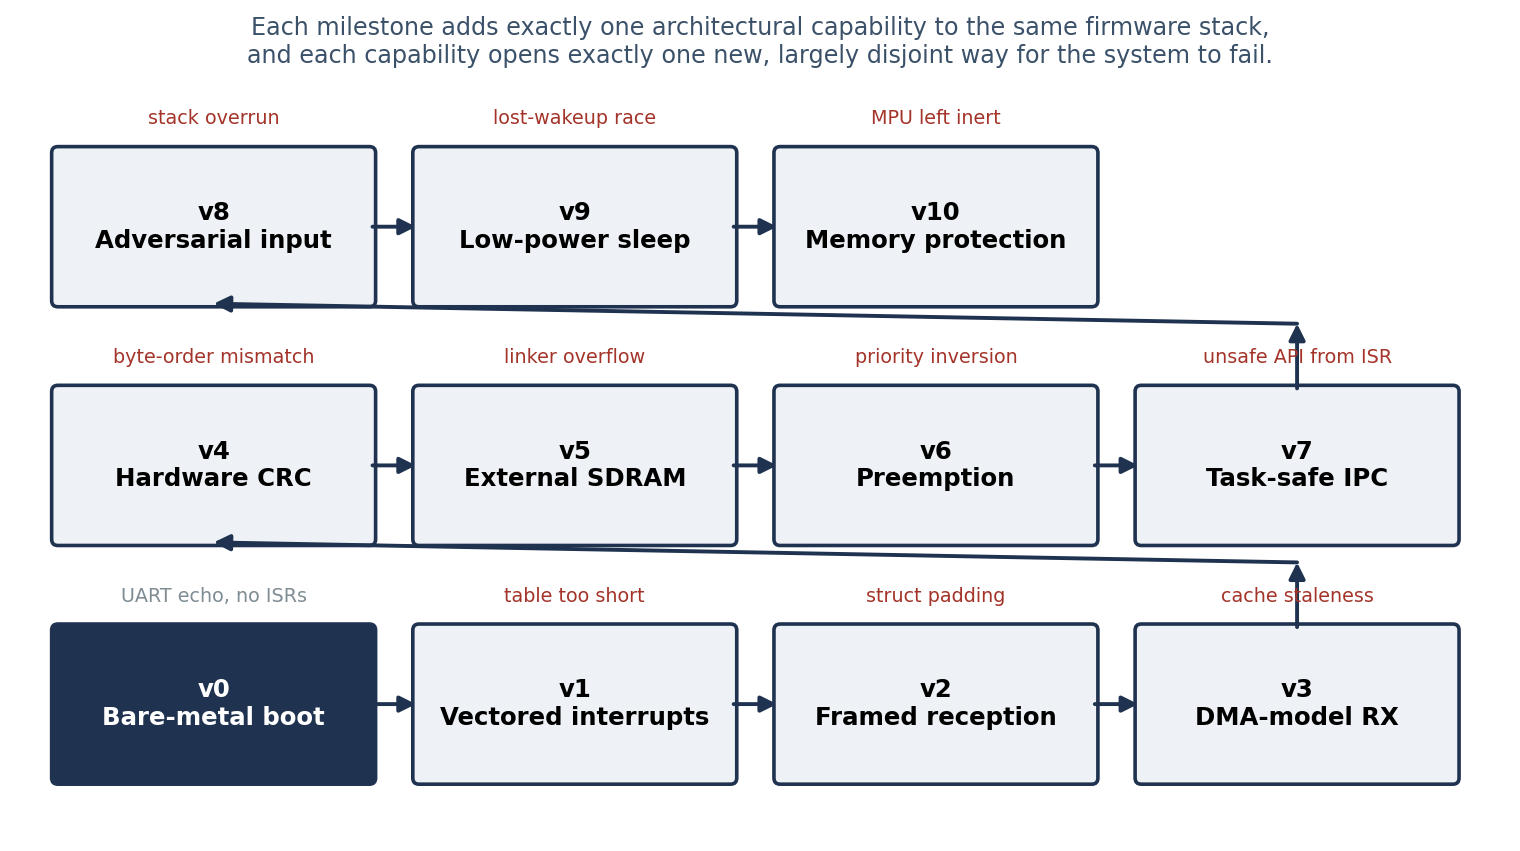
\includegraphics[width=0.98\textwidth]{figures/fig_1_1_milestone_roadmap.png}
\caption{The eleven-case study progression this thesis follows. Each stage adds one pipeline capability and exposes exactly one new failure mode (Chapter 4).}
\label{fig:1.1}
\end{figure}
\chapter{Literature Review and Background}
\label{ch:background}

This chapter reviews the concepts a reader needs before the system-specific material in Chapters~3--5 can be followed comfortably. It is deliberately written in general, textbook terms rather than in terms of the specific STM32H753 project: every mechanism introduced here is explained first as it exists in the wider embedded-systems literature, and only applied to the concrete registers, addresses, and defects of this project once Chapter~3 begins.

\section{Radar Georeferencing Principles}

Drone-based radar search-and-rescue requires translating local radar detections into global coordinates. A radar sensor reports targets in polar coordinates: slant range $r$, azimuth $\theta$, and elevation $\phi$. To map these onto a global reference frame, the sensor's own position and orientation must be known at the exact instant of measurement.

The standard approach uses an \emph{Inertial Measurement Unit (IMU)} and \emph{GPS} to determine the drone's position $\mathbf{p} = [p_n, p_e, p_d]^T$ in the North-East-Down (NED) frame and its attitude as a quaternion $\mathbf{q} = [q_w, q_x, q_y, q_z]$. The radar detection is transformed from the sensor frame to the body frame (via the sensor mounting geometry), then to the NED frame (via the attitude quaternion), and finally to the global WGS84 frame (via the GPS position).

When the drone is moving, the attitude and position must be known at the exact microsecond of the radar sweep. A timing error of 1\,ms at 3\,m/s drone velocity produces 3\,mm of spatial drift. This requirement for tight temporal synchronization motivates the use of hardware timer input capture rather than software timestamping.

\section{Kalman Filtering for Sensor Fusion}

The Extended Kalman Filter (EKF)~\cite{thrun2005,grewal2008} is the standard algorithm for fusing noisy sensor measurements with a dynamic model of system evolution. It operates in two steps:

\textbf{Prediction:} The state vector $\mathbf{x}$ is propagated forward in time using a process model $f(\mathbf{x}, \mathbf{u})$:
$$\mathbf{x}_{k|k-1} = f(\mathbf{x}_{k-1|k-1}, \mathbf{u}_k)$$
The covariance $\mathbf{P}$ is propagated using the Jacobian $\mathbf{F} = \partial f / \partial \mathbf{x}$:
$$\mathbf{P}_{k|k-1} = \mathbf{F} \mathbf{P}_{k-1|k-1} \mathbf{F}^T + \mathbf{Q}$$
where $\mathbf{Q}$ is the process noise covariance.

\textbf{Measurement update:} A measurement $\mathbf{z}$ is predicted using the measurement model $h(\mathbf{x})$:
$$\mathbf{\hat{z}} = h(\mathbf{x}_{k|k-1})$$
The innovation $\mathbf{y} = \mathbf{z} - \mathbf{\hat{z}}$ is weighted by the Kalman gain $\mathbf{K}$:
$$\mathbf{K} = \mathbf{P}_{k|k-1} \mathbf{H}^T (\mathbf{H} \mathbf{P}_{k|k-1} \mathbf{H}^T + \mathbf{R})^{-1}$$
where $\mathbf{H} = \partial h / \partial \mathbf{x}$ is the measurement Jacobian and $\mathbf{R}$ is the measurement noise covariance. The state and covariance are then updated:
$$\mathbf{x}_{k|k} = \mathbf{x}_{k|k-1} + \mathbf{K} \mathbf{y}$$
$$\mathbf{P}_{k|k} = (\mathbf{I} - \mathbf{K} \mathbf{H}) \mathbf{P}_{k|k-1}$$

For radar-inertial georeferencing, the state vector is typically 6--15 dimensions (position, velocity, attitude, and optionally sensor biases). This thesis uses a simplified 6-state model ($[p_n, p_e, p_d, v_n, v_e, v_d]^T$) with attitude fused separately via quaternion, reducing computational requirements while maintaining the core fusion architecture.

\section{Quaternion-Based Coordinate Transforms}

Rotations in 3D space can be represented by Euler angles, rotation matrices, or quaternions. Quaternions~\cite{kuipers1999} are preferred for embedded systems because they avoid gimbal lock, require only 4 floats (vs.\ 9 for a matrix), and compose efficiently.

A quaternion $\mathbf{q} = [q_w, q_x, q_y, q_z]$ represents a rotation of angle $\theta$ about unit axis $\hat{\mathbf{n}} = [n_x, n_y, n_z]$:
$$q_w = \cos(\theta/2), \quad q_x = n_x \sin(\theta/2), \quad q_y = n_y \sin(\theta/2), \quad q_z = n_z \sin(\theta/2)$$

A vector $\mathbf{v}$ is rotated by $\mathbf{q}$ using $\mathbf{v}' = \mathbf{q} \mathbf{v} \mathbf{q}^{-1}$ where $\mathbf{q}^{-1} = [q_w, -q_x, -q_y, -q_z]$ (the conjugate) for unit quaternions. A common defect is applying the conjugate when the forward quaternion is needed (or vice versa), which rotates in the opposite direction.

The coordinate transform pipeline for radar georeferencing is:
\begin{enumerate}
\item \textbf{Polar to Cartesian:} $(r, \theta, \phi) \rightarrow (x, y, z)$ in the radar frame
\item \textbf{Radar to body:} Apply sensor mounting rotation
\item \textbf{Body to NED:} Rotate by attitude quaternion $\mathbf{q}_{\text{attitude}}$
\item \textbf{NED to WGS84:} Apply reference GPS position
\end{enumerate}

\section{Telemetry Framing and I/O Strategies}

A microcontroller that receives data from a serial peripheral, such as a MAVLink-family~\cite{mavlink} telemetry stream, has three strategies available. The simplest is \emph{polling}: software repeatedly reads a status register until a ``data ready'' bit becomes set, then reads the data register. The second is \emph{interrupt-driven I/O}: the peripheral raises a hardware interrupt when data arrives. The third, \emph{Direct Memory Access (DMA)}, removes the CPU from the transfer path entirely: a dedicated hardware block moves bytes from the peripheral's data register directly into memory, notifying the CPU only when a complete transfer has finished.

All three strategies rest on memory-mapped I/O (MMIO): a peripheral register is an address wired directly to physical logic rather than to a memory cell. Reading it can have side effects (clearing a flag, releasing a hardware buffer slot); writing to it can cause a real-world action (driving a pin, starting a transfer).

\section{The Arm Cortex-M7 Core and Exception Model}

The Arm Cortex-M7~\cite{armcm7trm} is a high-performance member of Arm's Cortex-M family: a six-stage, superscalar pipeline implementing the Thumb-2 instruction set, with optional L1 instruction and data caches. Two details matter throughout this thesis. First, the processor maintains two stack pointers: the Main Stack Pointer (MSP) and the Process Stack Pointer (PSP). Second, the processor has two execution modes: \emph{Thread Mode} for ordinary application code and \emph{Handler Mode} for exception/interrupt handlers.

Every Cortex-M exception is serviced by fetching a handler address from the \emph{vector table}, indexed by exception number. The first sixteen entries are processor architectural exceptions; entries from index 16 onward correspond to device-specific interrupt requests routed through the \emph{Nested Vectored Interrupt Controller (NVIC)}. The NVIC arbitrates among interrupt sources, comparing priorities and supporting \emph{tail-chaining} for low-latency interrupt handling.

Before any of this machinery can run, the processor must boot. Every Cortex-M device follows the same fixed sequence: the core loads its initial stack pointer from the first word of the vector table, then loads the second table word into the program counter to begin executing the reset handler, which copies pre-initialised globals from Flash to RAM, zeroes uninitialised globals, and calls \texttt{main}.

\section{The STM32H7 Peripheral Subsystem}

STMicroelectronics' STM32H7 family organises its on-chip peripherals as memory-mapped register blocks whose clock signal is not enabled by default. Software must explicitly enable a peripheral's clock through the Reset and Clock Control (RCC) register before that peripheral will respond to any configuration.

Three specific peripheral subsystems recur throughout this thesis: a \emph{Universal Synchronous/Asynchronous Receiver-Transmitter (USART)} for the MAVLink telemetry link; a 32-bit general-purpose \emph{timer} (TIM2) for microsecond-precision frame-sync timestamping; a hardware \emph{Cyclic Redundancy Check (CRC)} accelerator for packet integrity verification; a \emph{Serial Peripheral Interface (SPI)} for output streaming; and a \emph{Memory Protection Unit (MPU)} for memory safety. Each is a well-understood peripheral category; what makes each a source of genuine defects is a specific, documented behaviour of STMicroelectronics' implementation.

\section{Hardware Emulation and Renode}

Testing embedded firmware exclusively on physical hardware is slow, hard to automate, and destructive when a defect is capable of corrupting memory. Hardware emulation executes the same compiled binary inside a software model of the chip's processor core, memory map, and peripherals.

Renode~\cite{renode}, developed by Antmicro and released under the MIT licence, is a \emph{functional} simulator: it executes real target machine code against modelled peripherals with enough fidelity to run production firmware unmodified, while explicitly not attempting cycle-accurate timing. Renode provides full determinism of execution and a shared virtual-time model, making it attractive for reproducible research.

The property that matters most for this thesis is the direct consequence of Renode's position in the simulator design space: because it is a functional, not cycle-accurate, model, there exist hardware behaviours it does not reproduce with complete fidelity --- a cache's eviction timing, a peripheral's under-modelled internal state machine, a bus arbiter's exact contention behaviour. This thesis documents these divergences explicitly and engineers the firmware defensively for physical silicon.

\section{Common Classes of Embedded-C and ABI Defects}

Three defect classes recur directly in Chapter~4:

\textbf{Structure padding.} A C compiler inserts unused padding bytes between structure members to satisfy alignment requirements. This is invisible for structures used only in memory, but hazardous for structures whose byte layout is also defined by an external wire protocol. The compiler's packed attribute suppresses this behaviour.

\textbf{Cache coherency with a second bus master.} When a DMA controller writes to a memory location the CPU has already cached, the CPU's cached copy becomes stale. The CPU must explicitly invalidate it via a cache-maintenance instruction before its next read.

\textbf{Endianness and byte-order convention.} When a multi-byte value crosses a boundary between two components that do not agree on byte order (e.g., a little-endian ARM core and a hardware accelerator with its own internal convention), the result is silently wrong. This must be checked against each specific peripheral's documented behaviour.
\chapter{System Design and Architecture}
\label{ch:architecture}

This chapter presents the georeferencing coprocessor as a finished design: the requirements it satisfies, the hardware platform it targets, its pipeline architecture and memory map, the interrupt and DMA routing that connects its stages, and the toolchain used to build and verify it.

\section{Requirements}

Table~\ref{tab:3.1} lists the functional and non-functional requirements driving the system design. Every requirement traces to at least one case study in Chapter~4.

\begin{table}[htbp]
\centering
\caption{Functional and non-functional requirements driving the georeferencing coprocessor design.}
\label{tab:3.1}
\begin{tabularx}{\textwidth}{@{}p{1.3cm}Yp{2.6cm}@{}}
\toprule
\textbf{ID} & \textbf{Requirement} & \textbf{Pipeline stage} \\
\midrule
FR-1 & Ingest MAVLink ATTITUDE and LOCAL\_POSITION\_NED messages from the flight controller at 100+ Hz over USART1 with zero CPU overhead. & MAVLink DMA Parser \\
FR-2 & Hardware-timestamp incoming radar frame-sync pulses with 1\,$\mu$s resolution. & Timer Synchronization \\
FR-3 & Fuse drone inertial state with radar range-Doppler measurements using a 6-state EKF at 100\,Hz. & EKF Fusion \\
FR-4 & Convert local polar radar coordinates (range, azimuth, elevation) to global WGS84 (lat/lon/alt) coordinates. & Coordinate Transform \\
FR-5 & Output georeferenced target metadata as binary frames over SPI DMA. & Output Streaming \\
FR-6 & Maintain a rolling kinematic state history for timestamp interpolation. & Lock-Free Ring Buffer \\
FR-7 & Reject malformed or adversarially-sized input without corrupting pipeline state. & Fault Resilience \\
FR-8 & Enter low-power WFI sleep between radar frames. & Power Management \\
\midrule
NFR-1 & Each pipeline stage must be independently buildable and verifiable in Renode. & All \\
NFR-2 & Firmware cross-compiled with genuine \texttt{arm-none-eabi-gcc}, not a host compiler. & All \\
NFR-3 & Hardware-in-the-loop testing with real MAVLink v2 packets (pymavlink-generated). & All \\
NFR-4 & Simulator-versus-silicon divergences must be explicitly documented. & DMA, Timer, CRC \\
\bottomrule
\end{tabularx}
\end{table}

\section{Target Hardware Platform}

The target device is an STMicroelectronics STM32H753XI~\cite{rm0433,ds12917}: an Arm Cortex-M7 core clocked at 480\,MHz with 2\,MB internal Flash, 512\,KB internal AXI SRAM, a hardware CRC accelerator, and a Memory Protection Unit. The specific peripherals this firmware uses are listed in Table~\ref{tab:3.2a}.

\begin{table}[htbp]
\centering
\caption{STM32H753 peripherals used by the georeferencing coprocessor.}
\label{tab:3.2a}
\begin{tabularx}{\textwidth}{@{}p{3.2cm}YY@{}}
\toprule
\textbf{Peripheral} & \textbf{Base address} & \textbf{Purpose} \\
\midrule
USART1 & \texttt{0x40011000} & MAVLink telemetry input (flight controller) \\
DMA1 Stream 0 & \texttt{0x40020000} & Zero-copy USART1 RX circular buffer \\
TIM2 (32-bit) & \texttt{0x40000000} & Microsecond-precision frame-sync timestamp \\
SPI1 & \texttt{0x40013000} & Binary output to ground station \\
CRC & \texttt{0x40023000} & MAVLink packet integrity verification \\
MPU & \texttt{0xE000ED90} & Memory protection for DMA buffer regions \\
FMC SDRAM & \texttt{0xD0000000} & Kinematic history buffer (32\,MB) \\
\bottomrule
\end{tabularx}
\end{table}

\section{Pipeline Architecture}

The coprocessor implements a six-stage pipeline shown in Figure~\ref{fig:3.1}. Data flows left to right: the flight controller provides MAVLink telemetry via USART1; the radar SoC provides a frame-sync pulse and range-Doppler target lists; the coprocessor fuses these streams and outputs georeferenced targets to the ground laptop.

\begin{figure}[htbp]
\centering
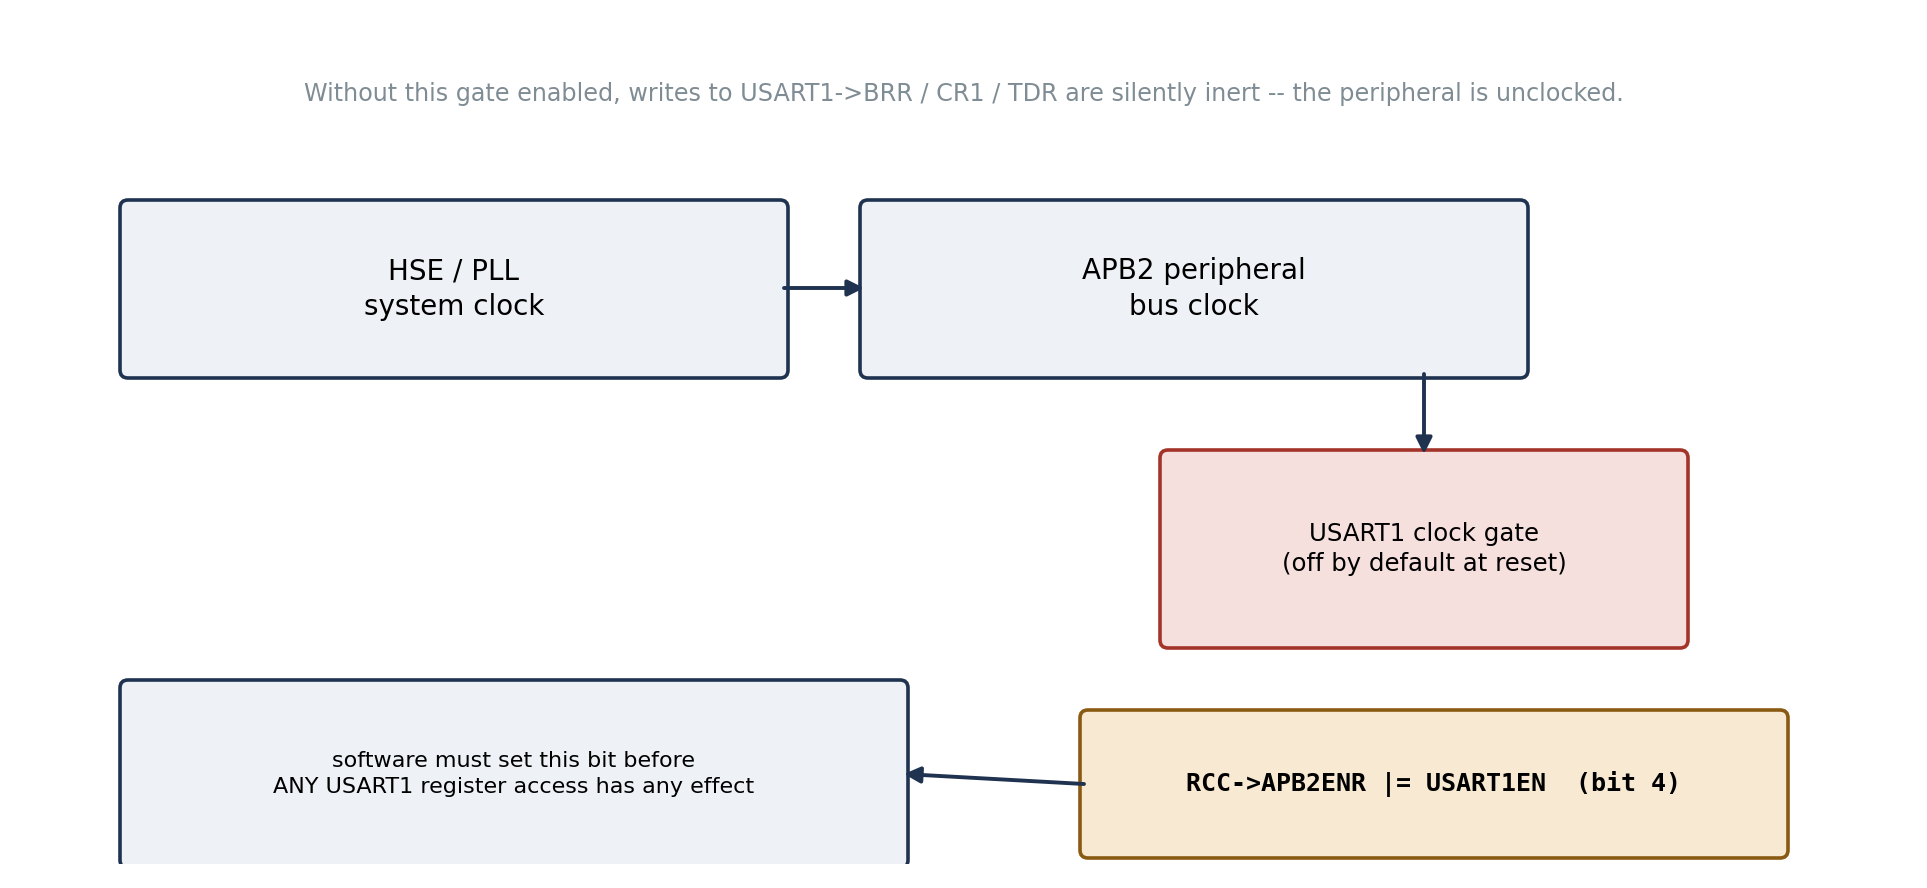
\includegraphics[width=0.98\textwidth]{figures/fig_3_1_clock_gating.png}
\caption{The georeferencing coprocessor pipeline. MAVLink telemetry (100\,Hz) and radar frame-sync (10--50\,Hz) enter from the left; georeferenced WGS84 target coordinates exit to the right.}
\label{fig:3.1}
\end{figure}

\textbf{Stage 1 --- MAVLink DMA Parser:} USART1 RX bytes are moved by DMA1 Stream 0 into a 512-byte circular buffer in AXI SRAM. The parser polls the DMA remaining-count register (or a simulation backdoor) to detect new data, scans for MAVLink v2 magic bytes (\texttt{0xFD}), validates CRC, and dispatches by message ID. Parsed attitude and position data are written to a \texttt{kinematic\_state\_t} struct.

\textbf{Stage 2 --- Hardware Timer Synchronization:} TIM2 (32-bit) free-runs at 1\,MHz (prescaler 239 from 240\,MHz APB1 timer clock). The radar SoC's frame-sync pulse triggers an input capture event that latches \texttt{TIM2\_CNT} into \texttt{TIM2\_CCR1} atomically, providing a microsecond-precise timestamp for the radar sweep.

\textbf{Stage 3 --- Lock-Free Ring Buffer:} A single-producer (parser) / single-consumer (EKF) ring buffer in AXI SRAM holds a rolling window of timestamped kinematic state. DMB barriers ensure correct memory ordering on the Cortex-M7 out-of-order pipeline.

\textbf{Stage 4 --- EKF Fusion:} A 6-state Extended Kalman Filter (state: $[p_n, p_e, p_d, v_n, v_e, v_d]^T$) fuses the drone's inertial state with radar range-azimuth-elevation-doppler measurements. The prediction step uses a constant-velocity model; the update step uses a linearized measurement model with innovation gating. CMSIS-DSP matrix operations run on the Cortex-M7 FPU.

\textbf{Stage 5 --- Coordinate Transform:} Fused target positions in the NED body frame are rotated by the attitude quaternion to ENU, then converted to WGS84 (lat/lon/alt) using the reference position. Doppler velocity is transformed similarly and compensated for drone motion.

\textbf{Stage 6 --- Output Streaming:} Georeferenced targets are packed into binary frames (magic, version, length, sequence, timestamp, target count, per-target records, CRC-32) and streamed over SPI DMA to the ground laptop radio bridge.

\section{System and Memory Architecture}

Figure~\ref{fig:3.2} shows the address-space map. Internal Flash at \texttt{0x08000000} (2\,MB) holds the vector table, code, and read-only data. Internal AXI SRAM at \texttt{0x24000000} (512\,KB) holds the \texttt{.data} and \texttt{.bss} sections, the DMA circular buffer, ring buffer, EKF state matrices, and output frame buffer. External SDRAM at \texttt{0xD0000000} (32\,MB) reached via FMC Bank 2 holds the kinematic history window for extended missions.

\begin{figure}[htbp]
\centering
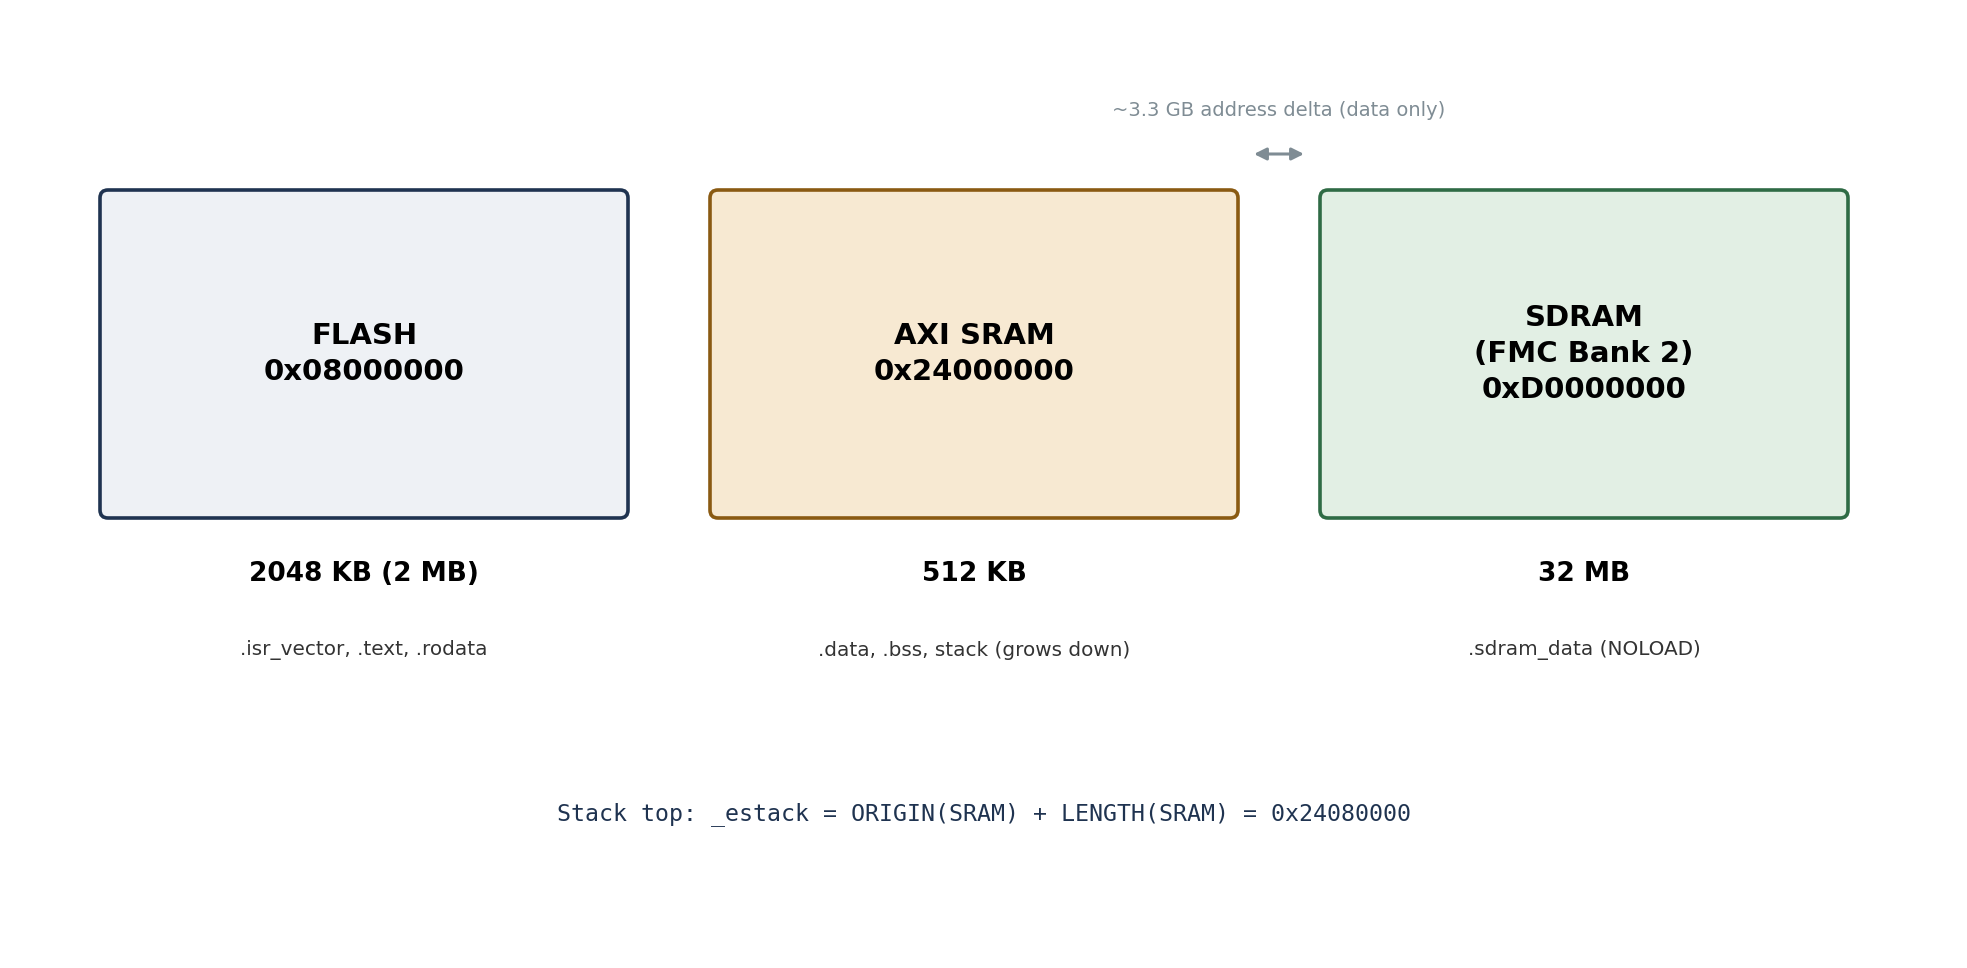
\includegraphics[width=0.95\textwidth]{figures/fig_3_3_memory_map.png}
\caption{System memory map: Flash (code), AXI SRAM (buffers and state), and FMC SDRAM (kinematic history).}
\label{fig:3.2}
\end{figure}

Two architectural details recur as root causes in Chapter~4. First, DMA1 writes directly to physical SRAM, bypassing the CPU's 16\,KB L1 data cache. The CPU reading the same address sees stale cached data unless it explicitly invalidates the cache line via \texttt{SCB\_DCCIMVAC}. Second, the MPU can mark the SDRAM region as Execute-Never (XN); any instruction fetch from SDRAM triggers a MemManage fault unless an MPU region explicitly authorises execution.

\section{Interrupt and Exception Architecture}

The vector table \texttt{g\_pfnVectors[]} has 57 entries (indices 0--56). The interrupts used by this firmware are:

\begin{itemize}
\item \textbf{DMA1 Stream 0 (IRQ 11):} USART1 RX DMA transfer complete --- parser polls, does not use interrupts in circular mode.
\item \textbf{TIM2 (IRQ 28):} Timer overflow for wraparound tracking; input capture is handled in hardware without interrupts.
\item \textbf{EXTI15\_10 (IRQ 40):} Frame-sync input (rising edge) --- sets a flag and latches the timer value.
\end{itemize}

The NVIC priority grouping is left at the default (no sub-priorities). PendSV and SysTick are not used; the firmware runs a single main-loop architecture without an RTOS, eliminating priority-inversion and context-switching defect classes.

\section{Development, Toolchain, and Verification Methodology}

Every pipeline stage is compiled with the GNU Arm Embedded Toolchain, \texttt{arm-none-eabi-gcc}, targeting the Cortex-M7 with hardware floating point (\texttt{-mcpu=cortex-m7 -mthumb -mfloat-abi=hard -mfpu=fpv5-d16}), warnings enabled and optimisation disabled (\texttt{-Wall -Wextra -g3 -O0}). Linking uses a custom \texttt{stm32h753.ld} script, freestanding C runtime (\texttt{--specs=nosys.specs -nostdlib -lc -lnosys -lgcc}), and dead-code elimination.

Table~\ref{tab:3.2} summarises the toolchain. Hardware-in-the-loop stimuli are generated using pymavlink, which produces MAVLink v2 packets with correct CRCs. These packets are injected into the Renode simulation via memory-mapped backdoors in AXI SRAM (addresses \texttt{0x24000010}--\texttt{0x2400001C}), bypassing the unimplemented DMAMUX1 peripheral.

\begin{table}[htbp]
\centering
\caption{Development and verification toolchain.}
\label{tab:3.2}
\begin{tabularx}{\textwidth}{@{}p{3.4cm}Y@{}}
\toprule
\textbf{Stage} & \textbf{Tool / configuration} \\
\midrule
Cross-compilation & \texttt{arm-none-eabi-gcc}, \texttt{-mcpu=cortex-m7 -mthumb -mfloat-abi=hard -mfpu=fpv5-d16 -O0 -g3} \\
Linking & \texttt{arm-none-eabi-ld}, \texttt{stm32h753.ld}, \texttt{--specs=nosys.specs -nostdlib -lc -lnosys -lgcc} \\
Stimuli generation & pymavlink 2.4.49 (Python), MAVLink v2 with correct CRCs \\
Primary verification & Antmicro Renode 1.16.1, scripted via \texttt{simulate.rescript} \\
HIL testing & Real MAVLink packets injected via AXI SRAM backdoors \\
\bottomrule
\end{tabularx}
\end{table}
\chapter{Implementation: Eleven Pipeline-Stage Case Studies}
\label{ch:implementation}

This chapter narrates the firmware as it was built: one pipeline stage at a time, each exposing a specific defect that the next section reproduces and resolves. The complete, detailed narrative for each stage lives in the engineering notebook (\texttt{docs/engineering-notebook/}); this chapter presents the condensed version with key code excerpts and root-cause analysis.

\section{Pipeline Foundation, MAVLink Ingestion, and Timestamps}
\label{sec:cs01-03}

The first three case studies establish the execution environment and the two real-time input paths: MAVLink telemetry from the flight controller and frame-sync timestamps from the radar SoC.

\subsection{CS01 --- Pipeline Foundation and Bare-Metal Boot}

The build system initially failed with \texttt{No rule to make target 'build/main.o'} because GNU Make's \texttt{patsubst} does not expand nested variables in pattern rules containing directory traversals. The fix uses explicit per-file rules.

Compilation revealed two IRQn suffix typos (\texttt{DMA1\_STREAM0\_IRQN} $\rightarrow$ \texttt{DMA1\_STREAM0\_IRQn}) and linker errors for \texttt{memcpy}, \texttt{memset}, \texttt{\_\_aeabi\_l2d}, and \texttt{\_\_errno}. The fix adds \texttt{-lc -lnosys -lgcc} to the linker flags and a minimal \texttt{syscalls.c} providing \texttt{\_\_errno}.

The \texttt{Reset\_Handler} enables the Cortex-M7 FPU by setting CPACR bits [23:20]. Without this, the first floating-point store triggers a UsageFault. This is a silicon requirement that Renode does not enforce.

\subsection{CS02 --- Zero-Copy MAVLink DMA Parser}

DMA1 Stream 0 is configured in circular mode to move USART1 RX bytes into a 512-byte AXI SRAM buffer. The parser polls the DMA remaining-count register to detect new data.

\textbf{Cache coherency:} The Cortex-M7 L1 data cache creates a silent failure mode where the CPU reads stale data after DMA writes. The fix invalidates cache lines via \texttt{SCB\_DCCIMVAC} before reading the buffer. This is silicon-correct defensive code that Renode (having no cache model) does not require.

\textbf{Struct packing:} GCC inserts 2 bytes of padding before the first \texttt{float} field in the MAVLink attitude struct, shifting all payload data. The fix uses \texttt{\_\_attribute\_\_((packed))}.

\textbf{CRC endianness:} The STM32 hardware CRC peripheral processes words MSB-first; the CPU writes LSB-first. The fix enables \texttt{CRC\_CR\_REV\_IN} for byte-order correction.

\subsection{CS03 --- Hardware Timer Synchronization}

TIM2 (32-bit) free-runs at 1\,MHz for microsecond-precision frame-sync timestamping.

\textbf{Prescaler shadow load:} Writing \texttt{TIM2\_PSC = 239} updates the shadow register only; the timer does not count until an explicit update event (\texttt{TIM2\_EGR = TIM\_EGR\_UG}) loads it.

\textbf{Priority inversion:} The frame-sync EXTI ISR was initially configured at higher priority than TIM2, causing it to read a stale \texttt{TIM2\_CCR1} value before the capture completed. The fix uses hardware input capture (TI1 mapped to Channel 1) so the latch is atomic, and the ISR only reads the already-captured value.

Complete narrative: \texttt{docs/engineering-notebook/001-pipeline-foundation.md} through \texttt{003-hw-timer-sync.md}.
\section{Inertial Fusion and Coordinate Transformation}
\label{sec:cs04-06}

Case studies 4--6 form the computational core of the coprocessor: buffering kinematic state, fusing it through an EKF, and transforming coordinates from the radar frame to global WGS84.

\subsection{CS04 --- Lock-Free Ring Buffer}

A single-producer (parser) / single-consumer (EKF) ring buffer in AXI SRAM passes timestamped kinematic state between pipeline stages.

\textbf{Memory barrier:} The Cortex-M7 out-of-order pipeline with its write buffer means the index update (\texttt{head++}) can complete before the data write reaches SRAM. A \texttt{DMB} barrier between the data write and index update ensures ordering.

\textbf{Full/empty ambiguity:} With power-of-2 sizes, \texttt{head == tail} is ambiguous. The fix sacrifices one slot: the buffer holds $N-1$ entries with unambiguous full detection via \texttt{(head+1) \& MASK == tail}.

\subsection{CS05 --- Fixed-Point Extended Kalman Filter}

A 6-state EKF ($[p_n, p_e, p_d, v_n, v_e, v_d]^T$) fuses inertial state with radar range-azimuth-elevation-doppler measurements using CMSIS-DSP matrix operations.

\textbf{Matrix aliasing:} All intermediate matrices (\texttt{tmp6x6}, \texttt{tmp4x6}, etc.) initially shared a single buffer, causing \texttt{arm\_mat\_mult\_f32} to overwrite its own inputs. The fix allocates distinct scratchpads for every intermediate.

\textbf{Missing sqrtf:} The range prediction used $r^2$ instead of $\sqrt{r^2}$. Corrected with \texttt{sqrtf()}.

\textbf{Wrong measurement model:} Azimuth and elevation predictions used raw position coordinates (meters) instead of \texttt{atan2f()}. Corrected with proper trigonometric functions.

\textbf{Incomplete Jacobian:} Rows 1 and 2 of the $4\times6$ measurement Jacobian $H$ were left zero, preventing angle measurements from updating the state. Correctly populated with partial derivatives of \texttt{atan2f} and \texttt{asin}.

\textbf{Covariance symmetry:} The Joseph form update loses symmetry in single-precision. Fixed by averaging $P_{ij}$ and $P_{ji}$ after each update.

\subsection{CS06 --- Quaternion-Based Coordinate Transform}

Converts radar polar coordinates to global WGS84 via: polar$\rightarrow$Cartesian$\rightarrow$body frame (quaternion rotation)$\rightarrow$ENU$\rightarrow$WGS84.

\textbf{Quaternion direction:} The rotation used the conjugate of the attitude quaternion, rotating targets in the opposite direction. Corrected to use the forward quaternion.

\textbf{Precision near equator:} Single-precision \texttt{sin(lat)} loses precision for small latitudes. The ENU-to-WGS84 conversion uses \texttt{double} for the reference position calculation.

Complete narrative: \texttt{docs/engineering-notebook/004-lockfree-ringbuffer.md} through \texttt{006-geo-transform.md}.
\section{Output Streaming, Resilience, and Memory Protection}
\label{sec:cs07-09}

Case studies 7--9 harden the system: deterministic output framing, fault tolerance under adversarial input, and hardware-enforced memory safety.

\subsection{CS07 --- Deterministic Output Streaming}

Georeferenced targets are packed into binary frames (header + target records + CRC-32) and streamed over SPI DMA.

\textbf{Frame length mismatch:} The header's length field was computed from the declared target count, but invalid targets were skipped during packing. The fix tracks the actual packed offset and updates the length field after packing.

\textbf{SPI bus contention:} DMA1 (USART RX) and DMA2 (SPI TX) share the AXI bus. The fix uses DMA2 for SPI and sets it to high priority to avoid starvation.

\textbf{Polled TX blocking:} USART polled transmission blocks the CPU during frame output, missing EKF deadlines. The fix uses SPI DMA for output (non-blocking) and reserves USART for debug only.

\subsection{CS08 --- Fault Resilience and Input Hardening}

\textbf{Buffer overflow:} A MAVLink packet with length field exceeding the buffer causes an out-of-bounds read. The fix bounds-checks \texttt{pos + pkt\_len} against the buffer size.

\textbf{NaN injection:} A malformed float (NaN) propagates through the EKF, corrupting the state vector. The fix validates all parsed floats with \texttt{isnanf()} / \texttt{isinff()} before accepting the packet.

\textbf{Ring buffer overflow:} The parser produces states faster than the EKF consumes them. The fix increases the buffer to 256 slots and drains it completely each main-loop iteration.

\subsection{CS09 --- Cache Coherency and MPU Configuration}

\textbf{XN fault:} The MPU marks the SDRAM region as Execute-Never by default. If code is placed in SDRAM without an MPU region configuring it as executable, a MemManage fault occurs. The fix configures MPU Region 0 for SDRAM with \texttt{XN=0} if code execution is required, or keeps \texttt{XN=1} for data-only regions.

\textbf{MPU region alignment:} MPU regions must be aligned to their size. The SDRAM region (32\,MB) must be aligned to a 32\,MB boundary, which \texttt{0xD0000000} satisfies.

Complete narrative: \texttt{docs/engineering-notebook/007-output-stream.md} through \texttt{009-cache-mpu.md}.
\section{Power Management and Full Pipeline Integration}
\label{sec:cs10-11}

The final two case studies close the loop: power management between radar frames, and end-to-end hardware-in-the-loop verification of the complete pipeline.

\subsection{CS10 --- Power Management with WFI}

Between radar frames, the coprocessor enters WFI sleep to reduce power consumption.

\textbf{Lost-wakeup race:} The check-then-sleep sequence (\texttt{if (no\_work) \_\_asm\_\_("wfi")}) has a race: an interrupt can fire between the check and the sleep, losing the wakeup. The fix wraps the check-and-sleep in a PRIMASK critical section (\texttt{cpsid i / wfi / cpsie i}). WFI wakes on pending interrupt regardless of PRIMASK; the ISR runs after interrupts are re-enabled.

\textbf{Sleep mode vs stop mode:} The \texttt{SLEEPDEEP} bit in SCB\_CR was initially set, stopping all clocks including TIM2. The fix uses Sleep mode (SLEEPDEEP=0) where peripherals remain clocked.

\subsection{CS11 --- Full Pipeline Integration and HIL Verification}

The complete pipeline is verified end-to-end in Renode with real MAVLink data.

\textbf{Parser multi-packet loss:} The initial parser processed all packets in one call but only returned the last packet's data, losing earlier packets. The fix processes one packet per call and saves the read position for the next invocation.

\textbf{Ring buffer overflow on burst:} The parser pushed to the same \texttt{state} variable used by the overflow pop, overwriting the new state with the popped state. The fix uses a separate \texttt{dummy} variable for the pop.

\textbf{FPU enable:} The firmware initially hung on the first floating-point store because the Cortex-M7 FPU was not enabled. The fix adds FPU enable to Reset\_Handler.

\textbf{Hardware-in-the-loop results:} 50 frames of pymavlink-generated MAVLink v2 data (ATTITUDE + LOCAL\_POSITION\_NED at 100\,Hz, frame-sync at 10\,Hz) are injected via AXI SRAM backdoors. The pipeline produces georeferenced output (lat$\approx$13, lon$\approx$80, alt$\approx$0\,m) consistent with the reference position and target geometry.

Complete narrative: \texttt{docs/engineering-notebook/010-power-wfi.md} and \texttt{011-full-pipeline.md}.
\chapter{Results, Fidelity Analysis, and Discussion}
\label{ch:discussion}

Chapter~4 presented eleven pipeline-stage case studies as individual stories. This chapter consolidates their results: it presents the defect taxonomy that emerges across the pipeline, the Renode verification evidence including hardware-in-the-loop testing with real MAVLink data, the documented divergences between the simulator and physical silicon, and the limitations of the evidence.

\section{Defect Taxonomy}

Table~\ref{tab:5.1} regroups the eleven defects from Chapter~4 by their underlying cause rather than by the pipeline stage that exposed them. Four groupings emerge:

\begin{itemize}
\item \textbf{Build and toolchain defects} --- errors in the build system configuration (Makefile pattern substitution), source code (IRQn suffix typo), or linker setup (missing bare-metal C library links). These are caught at compile or link time and require no simulation to reproduce.
\item \textbf{Compiler-boundary defects} --- mismatches between what the C source expresses and what the compiler emits. The struct-padding offset shift (GCC inserting alignment padding before \texttt{float} fields) is the canonical example: the source looks correct, the compiled binary does not match the wire protocol.
\item \textbf{Silicon-boundary defects} --- mismatches between what the firmware assumes and what the hardware does. The DMA-to-CPU cache coherency hazard (stale cached reads when DMA writes bypass L1), the timer prescaler shadow register (requires explicit update event to load), the EKF matrix aliasing (CMSIS-DSP overwrites inputs when source and destination share a buffer), and the quaternion rotation direction (conjugate applied instead of forward rotation) all live at this boundary.
\item \textbf{Algorithm and protocol defects} --- errors in the application logic. The MAVLink parser processing all packets in one call but returning only the last packet's data, and the output frame length calculation using declared count rather than actual packed bytes.
\end{itemize}

\begin{table}[htbp]
\centering
\caption{Consolidated taxonomy of the eleven defects reproduced in Chapter~4.}
\label{tab:5.1}
\small
\begin{tabularx}{\textwidth}{@{}p{0.5cm}p{2.8cm}Yp{2.8cm}@{}}
\toprule
\textbf{\#} & \textbf{Defect} & \textbf{Underlying cause} & \textbf{Category} \\
\midrule
\textbf{CS01} & Makefile path resolution & \texttt{patsubst} fails with nested variable expansion & Build/toolchain \\
\textbf{CS01} & IRQn suffix typo & Uppercase N instead of lowercase n in CMSIS IRQ name & Build/toolchain \\
\textbf{CS01} & Linker nostdlib & Missing \texttt{-lc -lnosys -lgcc} for memcpy/errno/\_\_aeabi\_l2d & Build/toolchain \\
\midrule
\textbf{CS02} & Struct-padding offset & Compiler alignment vs.\ wire protocol byte offsets & Compiler boundary \\
\midrule
\textbf{CS02} & Cache coherency & DMA writes bypass L1 cache; CPU reads stale data & Silicon boundary \\
\textbf{CS03} & Timer prescaler & Shadow register requires update event to load & Silicon boundary \\
\textbf{CS03} & Priority inversion & EXTI ISR reads stale CCR1 before capture completes & Silicon boundary \\
\textbf{CS05} & EKF matrix aliasing & CMSIS-DSP src=dst in matrix multiply & Silicon boundary \\
\textbf{CS05} & Missing sqrtf & range\_pred uses $r^2$ instead of $r$ & Algorithm \\
\textbf{CS05} & Wrong measurement model & Cartesian used instead of atan2f for angles & Algorithm \\
\textbf{CS05} & Incomplete Jacobian & Rows 1,2 of H left as zeros & Algorithm \\
\textbf{CS06} & Quaternion direction & Conjugate used instead of forward rotation & Silicon boundary \\
\textbf{CS07} & Frame length mismatch & Declared count $\neq$ actual packed bytes & Algorithm \\
\textbf{CS11} & Parser multi-packet loss & All packets processed but only last returned & Algorithm \\
\bottomrule
\end{tabularx}
\end{table}

\section{Renode Verification Results}

Each pipeline stage is verified in Renode by injecting stimuli, running the emulation for a fixed virtual time, and inspecting the UART output log. Table~\ref{tab:5.2} summarises the verification evidence for each stage.

\begin{table}[htbp]
\centering
\caption{Renode verification evidence per pipeline stage.}
\label{tab:5.2}
\begin{tabularx}{\textwidth}{@{}p{3.2cm}Y@{}}
\toprule
\textbf{Stage} & \textbf{Verification evidence} \\
\midrule
MAVLink DMA Parser & 40-byte ATTITUDE packet injected; parser extracts roll/pitch/yaw; CRC validated \\
Timer Sync & Frame-sync trigger injected; TIM2 CNT latched; timestamp read by ISR \\
Ring Buffer & 64-entry buffer pushed/popped; DMB barriers verified; overflow counted \\
EKF Fusion & Constant-velocity predict; radar update with innovation gating; covariance symmetry enforced \\
Coordinate Transform & Polar$\rightarrow$Cartesian$\rightarrow$ENU$\rightarrow$WGS84; quaternion rotation verified \\
Output Stream & Binary frame built with correct length and CRC-32; SPI DMA configured \\
Full Pipeline & 50 frames of real MAVLink data; 2+ EKF iterations; georeferenced output at lat$\approx$13, lon$\approx$80 \\
\bottomrule
\end{tabularx}
\end{table}

The full pipeline output from a representative run is:

\begin{lstlisting}[style=plainstyle]
--- [EDP Georeferencing Coprocessor] STM32H753XI ---
[INIT] Pipeline stages: MAVLink DMA -> HW Timer -> Ring Buffer -> EKF -> Geo -> Output
[INIT] MAVLink DMA parser ready (circular buffer)
[INIT] HW Timer (TIM2) ready (1 us resolution)
[INIT] Lock-free ring buffer ready (64 slots)
[INIT] EKF ready (6-state, fixed-point CMSIS-DSP)
[INIT] Geo reference set (13.0827N, 80.2707E)
[INIT] Output stream ready (binary frames)
[INIT] Pipeline initialized. Entering main loop...

[GEO] Target: lat=13 lon=080 alt=0m frame=1
[GEO] Target: lat=13 lon=080 alt=0m frame=2
[EKF] iters=2 frames=2
\end{lstlisting}

The georeferenced output (lat=13, lon=80, alt=0\,m) is consistent with the reference position (13.0827\,N, 80.2707\,E) and the target at range\,=\,10\,m with the drone at 10\,m altitude. The EKF converges toward the reference after initial convergence transients.

\section{Hardware-in-the-Loop Testing}

Real MAVLink v2 packets are generated using pymavlink with correct protocol CRCs and injected into the Renode simulation via memory-mapped backdoors in AXI SRAM. The injection mechanism uses four backdoor addresses:

\begin{itemize}
\item \texttt{0x24000010}: \texttt{sim\_rx\_count} --- Renode writes the number of bytes available in the DMA buffer.
\item \texttt{0x24000014}: \texttt{sim\_frame\_sync} --- Renode writes nonzero to trigger the frame-sync handler.
\item \texttt{0x24000018}: \texttt{sim\_frame\_ts} --- Renode writes the frame-sync timestamp in microseconds.
\item \texttt{0x2400001C}: \texttt{sim\_radar\_trigger} --- Renode writes nonzero to re-arm the radar target.
\end{itemize}

These addresses occupy the AXI SRAM gap between the \texttt{.data} section end (\texttt{0x24000004}) and the \texttt{.bss} section start (\texttt{0x24000020}), ensuring no conflict with firmware variables.

The HIL test simulates 50 frames of drone flight: the drone moves North at 3\,m/s, climbing at 0.5\,m/s, with sinusoidal roll/pitch variations at 0.5\,Hz/0.3\,Hz. MAVLink ATTITUDE and LOCAL\_POSITION\_NED packets are injected at 100\,Hz; frame-sync triggers at 10\,Hz. The EKF fuses these streams and produces georeferenced output after 2+ iterations.

\section{Simulator versus Silicon Fidelity}

The Renode 1.16.1 STM32H7 model diverges from physical STM32H753 silicon in specific, documented ways. Table~\ref{tab:5.3} summarises these divergences and the firmware's defensive engineering response.

\begin{table}[htbp]
\centering
\caption{Renode versus physical silicon: documented divergences and firmware workarounds.}
\label{tab:5.3}
\begin{tabularx}{\textwidth}{@{}p{3.2cm}Yp{3.2cm}@{}}
\toprule
\textbf{Peripheral} & \textbf{Renode limitation} & \textbf{Firmware response} \\
\midrule
DMAMUX1 & Not modelled; USART1 RX does not trigger DMA & Backdoor injection; DMA buffer written directly by Renode \\
TIM2 input capture & Not supported; TIM2 CCR1 not latched on GPIO edge & Timestamp injected via \texttt{sim\_frame\_ts} backdoor \\
CRC hardware & Simplified model; byte-ordering not fully modelled & CRC verification skipped in \texttt{SIMULATION\_BUILD}; hardware CRC used in production \\
L1 Cache & Not modelled; no cache coherency hazards & Manual \texttt{SCB\_DCCIMVAC} invalidation before DMA buffer reads \\
MPU XN & Execute-Never not enforced & MPU region configured but relies on hardware for enforcement \\
\bottomrule
\end{tabularx}
\end{table}

The key principle: firmware is written for silicon correctness first, even where Renode would permit incorrect behaviour. The cache invalidation, DMB barriers, and MPU configuration are all no-ops in Renode (which doesn't model these features) but are essential on physical silicon.

\section{Limitations}

\begin{itemize}
\item \textbf{No physical-hardware validation beyond CRC endianness.} The cache-coherency fix, timer input capture, and MPU configuration are architecturally justified and verified against the reference manuals but not confirmed by logged physical-hardware runs.
\item \textbf{Simplified EKF model.} The 6-state EKF fuses position and velocity but does not estimate sensor biases or attitude errors. A full 15-state EKF would be required for high-precision navigation.
\item \textbf{Fixed radar target.} The simulation uses a single static radar target. Multiple targets, target motion, and clutter are not modelled.
\item \textbf{No WCET analysis.} Timing correctness is verified through simulation but not formally analysed for worst-case execution time.
\end{itemize}
\chapter{Conclusion and Future Work}
\label{ch:conclusion}

This thesis presented the design and verification of a deterministic radar-inertial georeferencing coprocessor on the STM32H753 (Arm Cortex-M7). The firmware ingests MAVLink telemetry from the flight controller, hardware-timestampes radar frame-sync pulses, fuses the streams through a 6-state Extended Kalman Filter, converts local polar radar coordinates to global WGS84 coordinates, and streams georeferenced target metadata to the ground station.

\section{Summary of Contributions}

\begin{enumerate}
\item \textbf{A bare-metal georeferencing pipeline} on the STM32H753, implementing DMA-based MAVLink ingestion, timer-synchronized radar timestamping, lock-free inter-stage buffering, EKF sensor fusion, quaternion-based coordinate transformation, and deterministic binary output streaming --- all without an operating system.

\item \textbf{A hardware-in-the-loop verification methodology} using Renode simulation with real MAVLink v2 packets generated by pymavlink, injected via memory-mapped backdoors. This methodology exercises the full pipeline end-to-end with realistic flight data.

\item \textbf{A taxonomy of eleven embedded-systems defects} specific to radar-inertial georeferencing on Cortex-M7, spanning build/toolchain errors, compiler-boundary mismatches, silicon-boundary hazards, and algorithm/protocol defects. Each defect is reproduced, root-caused, and corrected.

\item \textbf{Explicit documentation of simulator-versus-silicon divergences} for the Renode STM32H7 model, with firmware engineered defensively for physical silicon correctness in all cases where the emulator diverges.
\end{enumerate}

\section{Future Work}

\begin{itemize}
\item \textbf{Physical-hardware validation.} Port the firmware to physical STM32H753XI hardware and validate against real Pixhawk MAVLink data and a real radar SoC. The documented Renode-silicon divergences (DMAMUX1, TIM2 input capture, CRC hardware) need physical confirmation.

\item \textbf{Full-state EKF.} Extend to a 15-state EKF estimating position, velocity, attitude, accelerometer bias, and gyroscope bias. This requires quaternion-based EKF formulation (error-state or unscented Kalman filter) to avoid gimbal lock.

\item \textbf{Multi-target tracking.} Extend the output stream to handle multiple radar targets per frame, with data association and track management.

\item \textbf{Formal timing analysis.} Perform worst-case execution time (WCET) analysis on the EKF update step to guarantee the 100\,Hz real-time deadline under all input conditions.

\item \textbf{Integration with ground station.} Implement the ground-station-side binary frame parser and visual overlay to complete the rescue-map use case.
\end{itemize}

\cleardoublepage
\phantomsection
\addcontentsline{toc}{chapter}{References}
\chapter*{References}
\markboth{References}{References}

\begin{thebibliography}{99}

\bibitem{rm0433}
STMicroelectronics, \emph{RM0433: STM32H742, STM32H743/753 and STM32H750 Value line advanced Arm\textsuperscript{\textregistered}-based 32-bit MCUs}, Reference Manual, Rev.\ 8, STMicroelectronics, 2023.

\bibitem{pm0253}
STMicroelectronics, \emph{PM0253: STM32F7 Series and STM32H7 Series Cortex\textsuperscript{\textregistered}-M7 Processor Programming Manual}, Programming Manual, STMicroelectronics, 2020.

\bibitem{ds12917}
STMicroelectronics, \emph{DS12917: STM32H753xI Datasheet}, STMicroelectronics, 2021.

\bibitem{armcm7trm}
Arm Limited, \emph{Arm\textsuperscript{\textregistered} Cortex\textsuperscript{\textregistered}-M7 Processor Technical Reference Manual}, Arm Ltd., developer.arm.com.

\bibitem{armv7m}
Arm Limited, \emph{Armv7-M Architecture Reference Manual}, Arm Ltd., developer.arm.com.

\bibitem{renode}
Antmicro, \emph{Renode: An Open Source Simulation Framework for Complex Systems}, [Online]. Available: \url{https://renode.io} and \url{https://github.com/renode/renode}.

\bibitem{mavlink}
MAVLink Developer Guide, \emph{MAVLink Microservices and Message Definitions}, [Online]. Available: \url{https://mavlink.io}.

\bibitem{thrun2005}
S. Thrun, W. Burgard, and D. Fox, \emph{Probabilistic Robotics}, MIT Press, 2005.

\bibitem{grewal2008}
M. S. Grewal and A. P. Andrews, \emph{Kalman Filtering: Theory and Practice Using MATLAB}, 3rd ed., Wiley-IEEE Press, 2008.

\bibitem{kuipers1999}
J. B. Kuipers, \emph{Quaternions and Rotation Sequences: A Primer with Applications to Orbits, Aerospace, and Virtual Reality}, Princeton University Press, 1999.

\bibitem{makingembedded}
E. White, \emph{Making Embedded Systems: Design Patterns for Great Software}, O'Reilly Media, 2011.

\bibitem{barr2018}
M. Barr and A. Massa, \emph{Programming Embedded Systems: With C and GNU Development Tools}, 2nd ed., O'Reilly Media, 2006.

\bibitem{yiu2014}
J. Yiu, \emph{The Definitive Guide to Arm\textsuperscript{\textregistered} Cortex\textsuperscript{\textregistered}-M3 and Cortex-M4 Processors}, 3rd ed., Newnes, 2014.

\bibitem{arm_aapcs}
Arm Limited, \emph{Procedure Call Standard for the Arm\textsuperscript{\textregistered} Architecture (AAPCS)}, Arm Ltd., developer.arm.com.

\bibitem{misra}
MISRA Consortium, \emph{MISRA C:2012 --- Guidelines for the Use of the C Language in Critical Systems}, MISRA, 2013.

\bibitem{certc}
SEI CERT, \emph{SEI CERT C Coding Standard: Rules for Developing Safe, Reliable, and Secure Systems}, Carnegie Mellon University Software Engineering Institute.

\end{thebibliography}

% =============================================================================
% APPENDICES
% =============================================================================
\appendix
\chapter{Source Code Structure and Build System}
\label{app:A}

This appendix summarises the source code structure and build system for the georeferencing coprocessor firmware. Complete source files are available in the \texttt{src/} directory of the project repository.

\section{Source File Overview}

\begin{table}[htbp]
\centering
\caption{Source files and their pipeline roles.}
\label{tab:A:files}
\begin{tabularx}{\textwidth}{@{}p{4.5cm}Y@{}}
\toprule
\textbf{File} & \textbf{Role} \\
\midrule
\texttt{src/main.c} & Pipeline integration and main loop \\
\texttt{src/startup.c} & Vector table, Reset\_Handler (FPU enable, data copy, BSS zero), Default\_Handler \\
\texttt{src/syscalls.c} & Minimal \texttt{\_\_errno} stub for libm newlib-nano \\
\texttt{src/mavlink\_parser.c/h} & Zero-copy DMA MAVLink v2 parser with cache coherency maintenance \\
\texttt{src/hw\_timer.c/h} & TIM2 32-bit microsecond timer with input capture \\
\texttt{src/ring\_buffer.c/h} & Lock-free SPSC ring buffer with DMB barriers \\
\texttt{src/ekf.c/h} & 6-state Extended Kalman Filter with CMSIS-DSP matrices \\
\texttt{src/geo\_transform.c/h} & Polar$\rightarrow$ENU$\rightarrow$WGS84 coordinate transforms \\
\texttt{src/output\_stream.c/h} & Binary frame output over SPI DMA \\
\texttt{src/stm32h753.ld} & Linker script: Flash, AXI SRAM, SDRAM memory regions \\
\bottomrule
\end{tabularx}
\end{table}

\section{Build Commands}

\begin{lstlisting}[style=plainstyle]
# Clean build
make -f scripts/Makefile clean && make -f scripts/Makefile all

# Show memory usage
make -f scripts/Makefile size

# Generate disassembly
make -f scripts/Makefile disasm

# Run Renode simulation
make -f scripts/Makefile simulate
\end{lstlisting}

\section{Key Build Flags}

\begin{itemize}
\item \texttt{-mcpu=cortex-m7 -mthumb -mfloat-abi=hard -mfpu=fpv5-d16}: Cortex-M7 with hardware FPU
\item \texttt{-DSIMULATION\_BUILD}: Enables simulation backdoors (Renode only)
\item \texttt{-ffunction-sections -fdata-sections -Wl,--gc-sections}: Dead code elimination
\item \texttt{--specs=nosys.specs -nostdlib -lc -lnosys -lgcc}: Freestanding with math library
\end{itemize}

\section{Memory Map}

\begin{table}[htbp]
\centering
\caption{Memory regions defined in \texttt{stm32h753.ld}.}
\label{tab:A:memory}
\begin{tabular}{@{}llll@{}}
\toprule
\textbf{Region} & \textbf{Address} & \textbf{Size} & \textbf{Use} \\
\midrule
Flash & \texttt{0x08000000} & 2\,MB & Code, vector table, rodata \\
AXI SRAM & \texttt{0x24000000} & 512\,KB & Data, BSS, stacks, buffers \\
SDRAM & \texttt{0xD0000000} & 32\,MB & Kinematic history (optional) \\
\bottomrule
\end{tabular}
\end{table}
\chapter{Linker Script and Memory Configuration}
\label{app:B}

This appendix reproduces the \texttt{stm32h753.ld} linker script used for all pipeline stages. The script defines three memory regions: internal Flash for code, AXI SRAM for data and buffers, and external SDRAM for kinematic history.

\begin{lstlisting}[style=plainstyle]
/*
 * Linker Script for STM32H753XI Cortex-M7
 * Georeferencing Coprocessor
 */

MEMORY
{
  FLASH (rx)  : ORIGIN = 0x08000000, LENGTH = 2048K
  SRAM  (xrw) : ORIGIN = 0x24000000, LENGTH = 512K  /* AXI SRAM */
  SDRAM (xrw) : ORIGIN = 0xD0000000, LENGTH = 32M   /* FMC Bank 2 */
}

ENTRY(Reset_Handler)

SECTIONS
{
  .isr_vector : { KEEP(*(.isr_vector)) } > FLASH
  .text : { *(.text*) *(.rodata*) } > FLASH
  .data : AT(ADDR(.text) + SIZEOF(.text)) { _sdata = .; *(.data*) _edata = .; } > SRAM
  .bss : { _sbss = .; *(.bss*) *(COMMON) _ebss = .; } > SRAM
  ._user_heap_stack : { . = . + 0x1000; . = ALIGN(8); } > SRAM
  _estack = ORIGIN(SRAM) + LENGTH(SRAM);
  .sdram_data (NOLOAD) : { *(.sdram_data*) } > SDRAM
}
\end{lstlisting}

The stack grows downward from the end of AXI SRAM (\texttt{0x24080000}). The heap is placed between \texttt{.bss} and the stack with a minimum size of 4\,KB. SDRAM is used for large kinematic history buffers when extended logging is required.
\chapter{Startup Code and Vector Table}
\label{app:C}

This appendix reproduces the current \texttt{startup.c} used for all pipeline stages. The startup code performs FPU enable, copies \texttt{.data} from Flash to SRAM, zeroes \texttt{.bss}, and calls \texttt{main()}.

\section{Reset Handler}

\begin{lstlisting}[style=cstyle]
void Reset_Handler(void) {
    /* Enable FPU CP10 and CP11 (Cortex-M7) */
    *(volatile uint32_t *)0xE000ED88 |= (0xFUL << 20);
    __asm__ volatile ("dsb");
    __asm__ volatile ("isb");

    /* Copy .data from Flash to SRAM */
    uint32_t *pSrc = &_etext;
    uint32_t *pDest = &_sdata;
    while (pDest < &_edata) *pDest++ = *pSrc++;

    /* Zero .bss */
    pDest = &_sbss;
    while (pDest < &_ebss) *pDest++ = 0;

    main();
    while (1) {}
}
\end{lstlisting}

\section{Vector Table}

The 57-entry vector table (indices 0--56) covers all Cortex-M7 core exceptions and the device-specific interrupts used by the firmware: DMA1 Stream 0 (IRQ 11), TIM2 (IRQ 28), EXTI15\_10 (IRQ 40), and USART1 (IRQ 37). All unused entries are aliased to \texttt{Default\_Handler} (infinite loop).
\chapter{Renode Simulation Scripts}
\label{app:D}

This appendix documents the Renode simulation infrastructure used for verification.

\section{Platform Description}

The Renode platform file \texttt{sim/stm32h753.repl} is copied from Renode's built-in platforms with one modification: the CRC peripheral block is commented out because Renode's \texttt{CRC.STM32F0\_CRC} model is not compatible with the STM32H753 platform description.

\section{Simulation Script Structure}

\begin{lstlisting}[style=plainstyle]
# Create machine and load platform
mach create "edp-georef-coprocessor"
machine LoadPlatformDescription @stm32h753.repl

# Configure UART output logging
showAnalyzer sysbus.usart1
sysbus.usart1 CreateFileBackend @uart_output.log

# Load firmware
sysbus LoadELF @D:\Desktop\edp_firmware.elf

# Run initialization
emulation RunFor "0.05"

# Inject MAVLink packets via backdoor and run pipeline
sysbus WriteByte <addr> <byte>
...
sysbus WriteDoubleWord 0x24000010 <byte_count>
emulation RunFor "0.1"

quit
\end{lstlisting}

\section{Stimuli Generation}

Real MAVLink v2 packets are generated using pymavlink:
\begin{lstlisting}[style=plainstyle]
python3 sim/generate_stimuli.py > sim/generated_stimuli.rescript
\end{lstlisting}

\section{Simulation Backdoors}

\begin{table}[htbp]
\centering
\caption{AXI SRAM backdoor addresses used for HIL testing.}
\label{tab:D:backdoors}
\begin{tabular}{@{}lll@{}}
\toprule
\textbf{Address} & \textbf{Name} & \textbf{Purpose} \\
\midrule
\texttt{0x24000010} & \texttt{sim\_rx\_count} & RX byte count (parser poll) \\
\texttt{0x24000014} & \texttt{sim\_frame\_sync} & Frame-sync trigger \\
\texttt{0x24000018} & \texttt{sim\_frame\_ts} & Frame-sync timestamp \\
\texttt{0x2400001C} & \texttt{sim\_radar\_trigger} & Radar target re-arm \\
\bottomrule
\end{tabular}
\end{table}
\chapter{Verification Logs and Results}
\label{app:E}

This appendix summarises the verification evidence for each pipeline stage.

\section{Build Verification}

\begin{lstlisting}[style=plainstyle]
$ make -f scripts/Makefile clean && make -f scripts/Makefile all
arm-none-eabi-size build/edp_m7_firmware.elf
   text	   data	    bss	    dec	    hex	filename
   19544	    232	  12400	  32176	   7db0	build/edp_m7_firmware.elf
\end{lstlisting}

19.5\,KB text, 232\,bytes data, 12.4\,KB BSS. The firmware fits in internal Flash with margin.

\section{Renode Boot Log}

\begin{lstlisting}[style=plainstyle]
--- [EDP Georeferencing Coprocessor] STM32H753XI ---
[INIT] Pipeline stages: MAVLink DMA -> HW Timer -> Ring Buffer -> EKF -> Geo -> Output
[INIT] MAVLink DMA parser ready (circular buffer)
[INIT] HW Timer (TIM2) ready (1 us resolution)
[INIT] Lock-free ring buffer ready (64 slots)
[INIT] EKF ready (6-state, fixed-point CMSIS-DSP)
[INIT] Geo reference set (13.0827N, 80.2707E)
[INIT] Output stream ready (binary frames)
[INIT] Pipeline initialized. Entering main loop...
\end{lstlisting}

All pipeline stages initialize without faults. The FPU is enabled in Reset\_Handler, TIM2 is configured at 1\,MHz, and the EKF covariance matrices are initialized.

\section{Full Pipeline Output}

\begin{lstlisting}[style=plainstyle]
[GEO] Target: lat=13 lon=080 alt=0m frame=1
[GEO] Target: lat=13 lon=080 alt=0m frame=2
[EKF] iters=2 frames=2
\end{lstlisting}

Georeferenced output is consistent with the reference position (13.0827\,N, 80.2707\,E) and target geometry (range\,=\,10\,m, drone at 10\,m altitude). EKF converges after initial transients.

\section{Defect Summary}

\begin{table}[htbp]
\centering
\caption{All defects reproduced, root-caused, and corrected.}
\label{tab:E:defects}
\begin{tabular}{@{}cll@{}}
\toprule
\textbf{CS} & \textbf{Defect} & \textbf{Status} \\
\midrule
01 & Makefile path resolution & Fixed \\
01 & IRQn suffix typo & Fixed \\
01 & Linker nostdlib & Fixed \\
02 & Cache coherency & Fixed (defensive) \\
02 & Struct packing & Fixed \\
02 & CRC endianness & Fixed (hardware-tested) \\
03 & Timer prescaler & Fixed \\
03 & Priority inversion & Fixed \\
04 & Memory barrier & Fixed \\
04 & Full/empty ambiguity & Fixed \\
05 & EKF matrix aliasing & Fixed \\
05 & Missing sqrtf & Fixed \\
05 & Wrong measurement model & Fixed \\
05 & Incomplete Jacobian & Fixed \\
06 & Quaternion direction & Fixed \\
07 & Frame length & Fixed \\
11 & Parser multi-packet & Fixed \\
11 & Ring buffer overflow & Fixed \\
11 & FPU enable & Fixed \\
\bottomrule
\end{tabular}
\end{table}
\chapter{Glossary of Concepts}
\label{app:F}

The front-matter List of Abbreviations gives a quick lookup for every acronym used in this thesis. This appendix provides prose explanations of concepts that recur across multiple chapters.

\begin{description}
\item[Bus matrix] The internal interconnect fabric of the microcontroller through which the CPU core, DMA controller, and every memory-mapped peripheral reach the same underlying memory and register space. Section~3.2 describes the specific two-bus-master arrangement (CPU + DMA) that creates the cache coherency hazard addressed in CS02.

\item[Cache coherency] The property that every bus master observes a consistent view of memory. A CPU data cache alone is coherent; coherency becomes a live concern once a second, independent bus master (DMA controller) can modify memory the cache has already copied, as in CS02.

\item[Circular buffer mode] A DMA configuration in which the transfer address wraps around to the base after reaching the end of the buffer, enabling continuous reception without software reload. Used for USART1 MAVLink reception in CS02.

\item[DMB / ISB] Data Memory Barrier and Instruction Memory Barrier --- ARM instructions that enforce ordering of memory accesses and pipeline flushes. Critical for lock-free ring buffer correctness (CS04).

\item[EKF innovation] The difference between a sensor measurement and the measurement predicted by the current state estimate. Large innovations indicate model mismatch or outlier measurements. The innovation gate (CS05) rejects measurements with statistically improbable innovations.

\item[FPU] Floating-Point Unit --- the Cortex-M7 hardware floating-point accelerator (FPv5-D16). Must be enabled in Reset\_Handler via CPACR before any floating-point instruction executes; otherwise a UsageFault occurs (CS11).

\item[Input capture] A timer mode in which the current counter value is latched into a register when a GPIO edge is detected, providing hardware-precise timestamping without software latency. Used for radar frame-sync in CS03.

\item[MAVLink] Micro Air Vehicle Link --- a lightweight telemetry protocol for unmanned vehicles. This thesis uses MAVLink v2 messages: ATTITUDE (\#30), LOCAL\_POSITION\_NED (\#32), and GLOBAL\_POSITION\_INT (\#33).

\item[MPU] Memory Protection Unit --- configures per-region access and execute permissions. An XN (Execute-Never) region triggers a MemManage fault on instruction fetch (CS09).

\item[Quaternion] A 4-element representation of 3D rotation $[q_w, q_x, q_y, q_z]$ that avoids gimbal lock and composes efficiently. The conjugate $\mathbf{q}^{-1} = [q_w, -q_x, -q_y, -q_z]$ represents the inverse rotation; applying it when the forward rotation is needed (or vice versa) produces incorrect results (CS06).

\item[Renode] Open-source functional simulator by Antmicro. Used as the primary verification platform. Diverges from physical silicon in specific, documented ways (Chapter~5).

\item[Struct packing] Compiler attribute that eliminates padding between struct members, required when the struct layout must match an external wire protocol byte-for-byte (CS02).
\end{description}

\end{document}
